\documentclass[12pt,brazil]{book}
\usepackage{babel}
\usepackage[utf8x]{inputenc}
\usepackage[top=2.5cm,left=2.5cm,bottom=2.5cm,right=2.5cm]{geometry}
\usepackage{url}
\usepackage{graphicx}
\usepackage{html}

\title{Genoslab Handbook}
\author{Pedro Kröger}

\begin{document}
\graphicspath{{figs/}}

\maketitle

\begin{htmlonly}
  Baixe a versão em pdf \htmladdnormallink{aqui}
  {http://genos.mus.br/handbook/genoslab-handbook.pdf}.
\end{htmlonly}

\tableofcontents

\part{Introdução}
\label{part:introducao}

% TODO
% \chapter{Como contribuir para esse documento}
% \label{sec:como-contribuir-para}

\part{Ferramentas}
\label{part:ferramentas}

\chapter{Git}
\label{cha:git}

\section{Introdução}
\label{sec:introducao}

O Git (o ``g'' é pronunciado como na palavra gato e não como ``jit'')
é um programa para controle de versão distribuído desenvolvido por
Linus Torvalds (o criador do Linux) e mantido por Junio C Hamano. A
página do git em \url{http://git.or.cz/} tem vários tutoriais e
manuais.

\section{Instalação}
\label{sec:instalacao-3}

Para instalar o git no debian execute o seguinte comando.

\begin{verbatim}
aptitude install git-core git-completion git-doc git-gui gitk ssh
\end{verbatim}

É uma boa idéia configurar o git para usar o seu nome e email:

\begin{verbatim}
git config --global user.name "Seu Nome"
git config --global user.email "seu@email.com.br"
\end{verbatim}

\section{Repositórios do genos}
\label{sec:acesso-de-escrita}

O genos mantém diversos repositórios listados em
\url{git.genos.mus.br}. Para ter acesso de escrita você precisa criar
uma chave pública de criptografia. Para isso rode o comando:

\begin{verbatim}
ssh-keygen -t rsa
\end{verbatim}

Esse comando vai fazer uma série de perguntas como o tamanho da chave,
seu nome e email, etc. Se você não souber a resposta para alguma
pergunta não precisa se preocupar, o valor padrão deve ser o
suficiente. Quando ele pedir uma passphrase, certifique-se que você
não vai esquecê-la! A chave pública vai ser geradad no arquivo
\texttt{~/.ssh/id\_rsa.pub}. Para ter acesso de escrita nos
repositórios do genos envie o arquivo para Pedro Kroger.

Se você enviou a chave pública e seu acesso foi liberado, você pode
baixar um projeto no repositório do genos com o comando abaixo:

\begin{verbatim}
git clone ssh://cons@genos.mus.br/repos/<nome do projeto>
\end{verbatim}

Por exemplo, para baixar o projeto analise-harmonica você deve
digitar:

\begin{verbatim}
git clone ssh://cons@genos.mus.br/repos/analise-harmonica.git
\end{verbatim}

Contudo, se você não tem acesso de escrita ao repositório, ou seja,
não tem permissão para modificar o repositório diretamente, você ainda
pode baixar um projeto e contribuir mudanças (veja a seção
\ref{sec:enviando-patches}). Para isso baixe o repositório com o
comando abaixo:

\begin{verbatim}
git clone http://genos.mus.br/repos/<nome de repositório>
\end{verbatim}

\section{Comandos básicos}
\label{sec:comandos-basicos}

Você deve gravar suas mudanças com

\begin{verbatim}
git commit
\end{verbatim}

E enviar suas mudanças para o repositório central com o comando:

\begin{verbatim}
git push
\end{verbatim}

Para atualizar sua cópia local, ou seja, para baixar as mudanças que
outros tenham feito no repositório, use o comando:

\begin{verbatim}
git pull
\end{verbatim}

Revertendo mudanças que não foram enviadas.

\begin{verbatim}
git checkout -f
\end{verbatim}

\section{Usando diferentes ramos}
\label{sec:usando-o-git}

Para ver os ramos do repositório basta usar o comando

\begin{verbatim}
git branch
\end{verbatim}

Para mudar de ramo usa-se o comando

\begin{verbatim}
git checkout
\end{verbatim}

Mudando do ramo master para novo-ramo:

\begin{verbatim}
git checkout novo-ramo
\end{verbatim}

Conferindo o novo ramo:

\begin{verbatim}
git branch
  master
* novo-ramo
\end{verbatim}

Para criar um novo ramo e mudar para ele automaticamente usa-se

\begin{verbatim}
git checkout -b novo-ramo
\end{verbatim}

Para enviar um novo ramo para o repositório remoto:

\begin{verbatim}
git push origin ramo-local:ramo-remoto
\end{verbatim}

Para listar os ramos em um repositório remoto

\begin{verbatim}
git branch -r
\end{verbatim}

Para baixar um ramo no repositório remoto usa-se \texttt{git branch}
com a opção \texttt{--track}, indicando qual o nome do ramo local e o
nome do ramo remoto. É uma boa prática ter o mesmo nome para os ramos
local e remoto.

\begin{verbatim}
git branch --track novo-ramo origin/novo-ramo
\end{verbatim}

O nome \texttt{origin} nada mais é que um alias para a localização de
um repositório. Essa informação fica armazenada no arquivo
\texttt{.git/config} dentro do repositório. O trecho do
\texttt{.git/config} referente a configuração de \texttt{origin} pode
ser vista abaixo:

\begin{verbatim}
[remote "origin"]
        url = ssh://cons@genos.mus.br/repos/teste.git
        fetch = +refs/heads/*:refs/remotes/origin/*
\end{verbatim}

Veja na seção \ref{sec:o-arquivo-config} outras possibilidades de uso
para o arquivo \texttt{.git/config}.

Para manter os ramos atualizados, \texttt{git pull} e \texttt{git
  push} devem ser suficientes. O Git mantém cada ramo separado sem
interferir no outro. Contudo, mudanças sem commit vão aparecer em
todos os ramos.

\section{Configuração}
\label{sec:configuracao}

\subsection{Usando abreviações}
\label{sec:usando-abreviacoes}

Eu sugiro que você coloque algo como a linha abaixo no seu
\texttt{~/.bashrc}.

\begin{verbatim}
export repos=ssh://cons@genos.mus.br/repos
\end{verbatim}

Desse modo você poderá baixar um projeto de uma maneira mais fácil:

\begin{verbatim}
git clone $repos/analise-harmonica.git
\end{verbatim}

\subsection{O arquivo config}
\label{sec:o-arquivo-config}

Você pode configurar o arquivo \texttt{.git/config} de um repositório
local para usar nomes abreviados. Isso é particularmente útil se está
usando mais de um repositório ou ramos diferentes.

\begin{verbatim}
cat >>.git/config <<EOF
[remote "public-repo"]
        url = ssh://yourserver.com/~you/proj.git
EOF
\end{verbatim}

Você pode fazer a mesma coisa com \texttt{git remote}:

\begin{verbatim}
git remote add public-repo ssh://example.com/project.git
\end{verbatim}

\subsection{Saída colorida}
\label{sec:saida-colorida}

Se você é viciado em saída colorida vai querer executar os comandos abaixo:

\begin{verbatim}
git config --global color.diff auto
git config --global color.status auto
git config --global color.branch auto
\end{verbatim}

\section{Enviando patches}
\label{sec:enviando-patches}


\part{Programas de áudio}
\label{part:programas-de-audio}

\chapter{CLM---Common Lisp Music}
\label{cha:clm-common-lisp}

\section{Pré-requisitos}
\label{sec:pre-requisitos}

Para compilar o CLM você precisará do gcc (o compilador C do projeto
GNU) e outras ferramentas instaladas. Além disso, o CLM não é um
programa auto-contido como o Csound. Ele é na verdade uma biblioteca
de funções Lisp. Para utiliza-lo você precisará de um compilador Lisp.
Eu recomendo o SBCL. Finalmente, você precisará de um bom editor. Eu
recomendo o Emacs com o Slime. O comando abaixo deve instalar tudo que
você precisa para começar:

\begin{verbatim}
aptitude install gcc emacs22 slime sbcl
\end{verbatim}

\section{Instalação}
\label{sec:instalacao}

Infelizmente não existe um pacote do CLM para o debian, então teremos
que instala-lo manualmente. Além disso, vamos instalar de uma maneira
que é mais fácil mas não é necessariamente robusta. Contudo essa
maneira é suficiente para você iniciar no programa. No futuro veremos
maneiras mais robustas de instalar o CLM.

Baixe a última versão do CLM no site do projeto em
\url{http://ccrma.stanford.edu/software/clm/} e descompacte o tar.gz
em um diretório. O diretório clm-3 será criado quando o arquivo for
descompactado. Os comandos abaixo efetuam essas operações:

\begin{verbatim}
wget ftp://ccrma-ftp.stanford.edu/pub/Lisp/clm-3.tar.gz
tar -xzf clm-3.tar.gz
\end{verbatim}

Observe que dentro do diretório clm-3 existem diversos arquivos. Os
arquivos com a extensão *.ins definem instrumentos do CLM e são os que
nos interessam. O próximo passo é compilar o CLM. Para isso inicie o
emacs e slime com \texttt{M-x slime}. O REPL (\textit{Read Eval Print
  Loop}) é o modo interativo de Lisp. Nele você pode digitar
expressões e obter resultados. Para programas maiores é desconfortável
entrar expressões no REPL, mas para testar coisas ele é bastante útil.
No REPL digite o comando abaixo para definir o diretório padrão. Esse
diretório deve ser onde você descompactou o CLM.

\begin{verbatim}
(setf *default-pathname-defaults* #p"/home/kroger/clm-3/")
\end{verbatim}

A figura abaixo mostra o resultado dessa expressão no emacs.

\begin{htmlonly}
  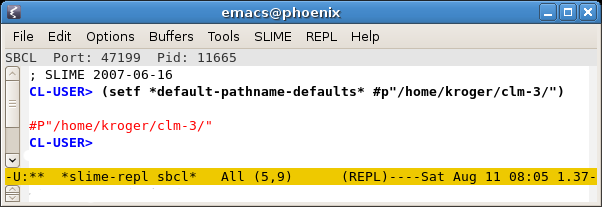
\includegraphics{slime1}
\end{htmlonly}

\begin{latexonly}
  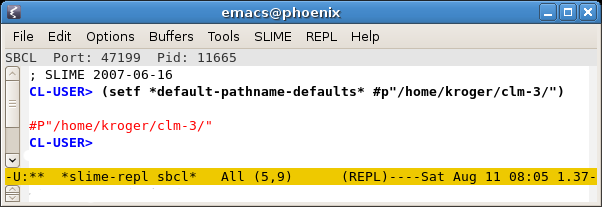
\includegraphics[scale=.5]{slime1}
\end{latexonly}

Agora rode o comando abaixo para compilar o CLM.

\begin{verbatim}
(load "all.lisp")
\end{verbatim}

\section{Uso básico}
\label{sec:uso-basico}

Tendo compilado o CLM você pode carregar e usar instrumentos definidos
nos arquivos *.ins. Por exemplo, o arquivo v.ins define um instrumento
de nome ``fm-violin'' que sintetiza um violino usando FM. Antes de
carregar os arquivos com instrumentos é necessário compilá-los. Você
pode fazer isso em uma  única etapa:

\begin{verbatim}
(load (compile-file "v.ins"))
\end{verbatim}

Contudo você só precisa compilar os instrumentos uma única vez (a
menos que o instrumento seja modificado). Se o instrumento já tiver
sido compilado, é só carrega-lo com:

\begin{verbatim}
(load "v")
\end{verbatim}

Finalmente, você pode usar o instrumento com o comando abaixo:

\begin{verbatim}
(with-sound () (fm-violin 0 1 440 .1)) 
\end{verbatim}

\section{Para saber mais}
\label{sec:para-saber-mais}

Para saber mais sobre a instalação do CLM veja o arquivo README.clm.
O manual está no arquivo clm.html. Ambos estão no diretório do CLM.

\chapter{Nyquist}
\label{cha:nyquist}

\section{Instalação}
\label{sec:instalacao-1}

Para instalar o nyquist é só usar o aptitude:

\begin{verbatim}
aptitude install nyquist
\end{verbatim}

O binário do nyquist se chama \texttt{ny}. Se você digitar \texttt{ny}
no terminal um prompt interativo vai abrir e esperar por comandos.
Você pode digitar algo simples para testar se o programa está
funcionando. O comando abaixo vai tocar um dó central:

\begin{verbatim}
(play (osc 60))
\end{verbatim}

\begin{htmlonly}
  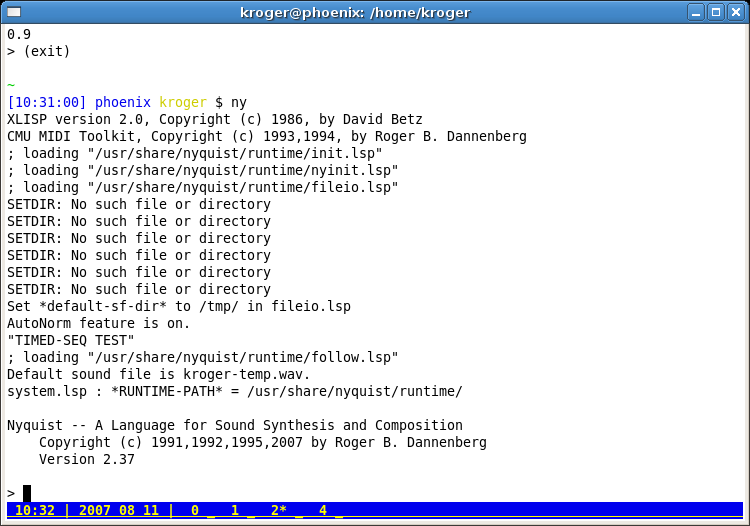
\includegraphics{ny1}
\end{htmlonly}

\begin{latexonly}
  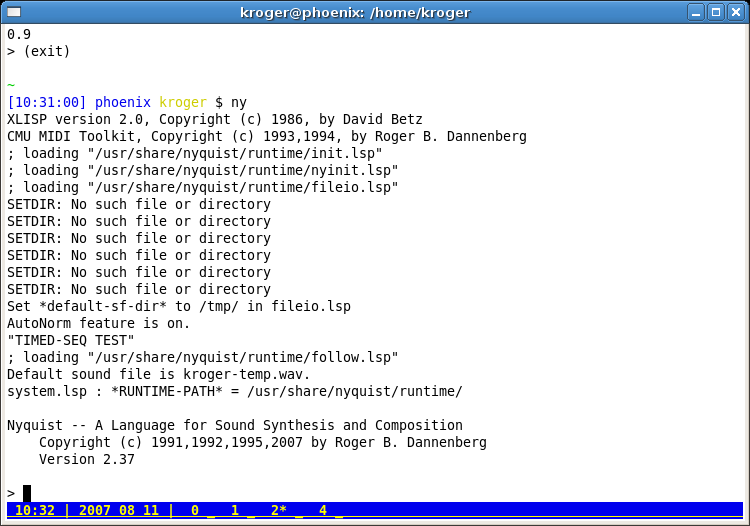
\includegraphics[scale=.5]{ny1}
\end{latexonly}

Nyquist vem com uma IDE escrita em Java. Ela ainda não está no pacote
do debian. Eu confesso que essa IDE não é muito boa. Eu prefiro
desenvolver usando o bom e velho Emacs. O problema é que não existe um
modo específico para o Nyquist, e se você configurar o emacs
globalmente para o Nyquist vai interferir com o Slime. A solução que
eu dou por enquanto é salvar \htmladdnormallink{essas
  configurações}{http://www.audacity-forum.de/download/edgar/nyquist/nyquist-doc/examples/emacs/main.html}
em um arquivo nyquist.el, carregar o emacs sem as configurações de
usuario (ou seja, sem carregar o .emacs) e carregar o arquivo
nyquist.el quando o emacs iniciar. Esse método é meio gambiarrico, mas
até ter uma solução adquada parece ser a melhor maneira.

\chapter{SuperCollider}
\label{cha:supercollider}

O SuperCollider é uma linguagem de programação para síntese de áudio
em tempo real e composição algorítmica. A página do programa fica em
\url{http://supercollider.sourceforge.net}.

\section{Instalação}
\label{sec:instalacao-2}

Para instalar o supercollider no debian é só executar o comando
abaixo:

\begin{verbatim}
aptitude install supercollider supercollider-doc supercollider-server
\end{verbatim}

\section{Uso básico}
\label{sec:uso-basico-1}

Nós vamos usar o SuperCollider dentro do Emacs. Para ativar o modo
sclang que permite interagir com o SC coloque a seguinte linha no seu
\texttt{~/.emacs}:

\begin{verbatim}
(require 'sclang)
\end{verbatim}

O SuperCollider usar o jack para entrada e saida, então tenha certeza
de te-lo rodando antes de carregar o SC. Inicie o emacs e carregue o
modo sclang:

\begin{verbatim}
M-x sclang-start
\end{verbatim}

O emacs vai abrir dois \textit{buffers}, um chamado *SCLang:Workspace*
e outro *SCLang:PostBuffer*. No Workspace você pode digitar comandos
do SC. Os resultados dos comandos vão aparecer no PostBuffer.

O menu SCLang no emacs tem diversos comandos para lidar com o SC. O
mais importante é como parar um som que esteja tocando. Você pode
acessá-lo em SCLang$\leftarrow$Stop Main no menu, ou pelo teclado com
\texttt{C-c C-s}. Para computar uma linha de código use \texttt{C-c
  C-c } (ou \textit{Evaluate Line} no menu).

Para iniciar o servidor, digite a linha abaixo e, com o cursor em
qualquer lugar da linha, digite \texttt{C-c C-c}:

\begin{verbatim}
s = Server.local.boot;
\end{verbatim}

Agora compute a linha abaixo para tocar um lá continuamente (lembre de
usar o \texttt{C-c C-s} para parar o som).

\begin{verbatim}
{SinOsc.ar(442, 0, 0.2) }.play;
\end{verbatim}

Finalmente, para demonstrar o poder expressivo do SuperCollider, veja
o que é possível de fazer com uma única linha de código:

\begin{verbatim}
play{SinOsc.ar(OnePole.ar(Mix(LFSaw.ar([1,0.99],[0,0.6],2000,2000).trunc([400,600])*[1,-1]),0.98)).dup*0.1};
\end{verbatim}

\section{Para saber mais}
\label{sec:para-saber-mais-1}

O site do SuperCollider tem vários tutoriais na página
\url{http://supercollider.sourceforge.net/learning}.

\end{document}
